% The unit square with oriented colored edges mapped by c to a curved 2-cell.
% Source: book/tex/diffgeo/stokes.tex (§ Cells).
\documentclass[border=2mm]{standalone}
\usepackage{tikz}\usetikzlibrary{arrows.meta}\usepackage{amssymb}
\begin{document}
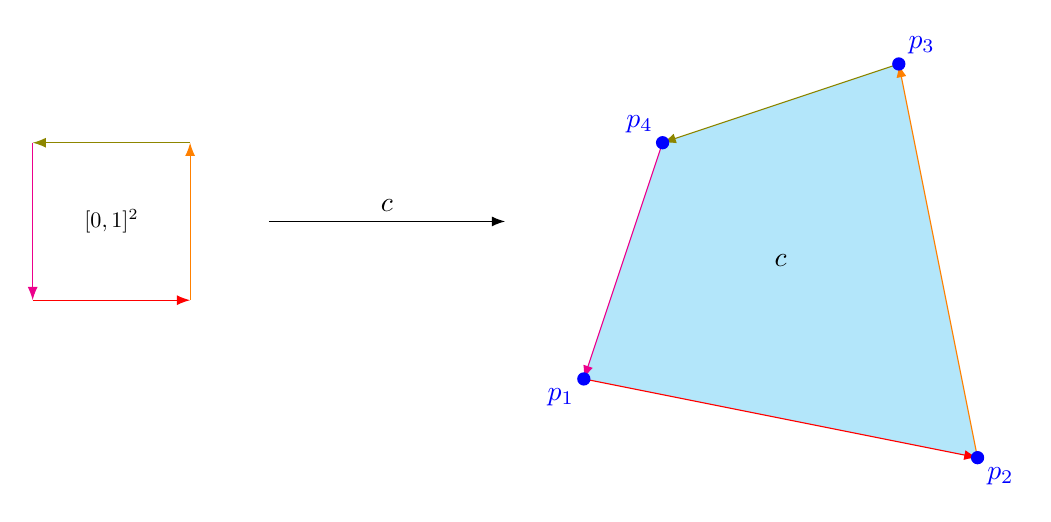
\begin{tikzpicture}[>={Latex}]
  \draw[red,->] (0,0)--(2,0); \draw[orange,->] (2,0)--(2,2);
  \draw[olive,->] (2,2)--(0,2); \draw[magenta,->] (0,2)--(0,0);
  \node at (1,1) {\scalebox{0.8}{$[0,1]^2$}};
  \draw[->] (3,1)--(6,1) node[midway,above]{$c$};
  \coordinate (p1) at (7,-1);\coordinate (p2) at (12,-2);\coordinate (p3) at (11,3);\coordinate (p4) at (8,2);
  \fill[cyan!30] (p1)--(p2)--(p3)--(p4)--cycle;
  \draw[red,->] (p1)--(p2);\draw[orange,->] (p2)--(p3);\draw[olive,->] (p3)--(p4);\draw[magenta,->] (p4)--(p1);
  \fill[blue] (p1)circle(2.4pt) node[below left]{$p_1$};\fill[blue] (p2)circle(2.4pt) node[below right]{$p_2$};
  \fill[blue] (p3)circle(2.4pt) node[above right]{$p_3$};\fill[blue] (p4)circle(2.4pt) node[above left]{$p_4$};
  \node at (9.5,0.5) {$c$};
\end{tikzpicture}
\end{document}
